% \begin{frame}
%     \frametitle{Visualizzare ed Elaborare documenti XML}
%     \addtocounter{nframe}{1}
    
%     %\begin{center}
%     %    
\includegraphics[width=.2\textwidth]{../imgs/tei-r.pdf}
%     %\end{center}
%     %\textit{In parte già disponibili nei moduli TEI di base}

%      \begin{block}{Perché visualizzare il testo}
%     %     \emph{Per la critica testuale indispensabili i moduli}
%          \begin{itemize}
%             \item  Controllare la codifica e correggere i refusi
%              \item Assicurarsi che tutto sia stato trascritto correttamente
%              \item Mostrare il testo a persone che non conoscono XML-TEI
%              \item Disporre di una versione del lavoro fuibile
%         \end{itemize}
%      \end{block}
    
% \end{frame}



\begin{frame}
    \frametitle{Fondamenti Extensible Stylesheet Language}
    \addtocounter{nframe}{1}
    
    %\begin{center}
    %    
\includegraphics[width=.2\textwidth]{../imgs/tei-r.pdf}
    %\end{center}
    %\textit{In parte già disponibili nei moduli TEI di base}

     \begin{block}{eXtensible Stylesheet Language (XSL)}
    %     \emph{Per la critica testuale indispensabili i moduli}
         \begin{itemize}
            \item  Specifica del W3C che descrive un metodo per la visualizzazione e manipolazione dei documenti XML
             \item Maggiore controllo sulla presentazione dei dati XML
             \item Generazione di layout complessi e composti
        \end{itemize}
     \end{block}
    
\end{frame}


\begin{frame}
    \frametitle{Fondamenti Extensible Stylesheet Language}
    \addtocounter{nframe}{1}
    
    %\begin{center}
    %    
\includegraphics[width=.2\textwidth]{../imgs/tei-r.pdf}
    %\end{center}
    %\textit{In parte già disponibili nei moduli TEI di base}

     \begin{block}{XSL incorpora tre linguaggi}
    %     \emph{Per la critica testuale indispensabili i moduli}
         \begin{itemize}
            \item \textbf{XSL Transformations (XSL-T)}: \textit{trasformazione di un documento XML in un altro tipo di documento} (es.: HTML)
            \item \textbf{XSL Formatting Objects (XSL-FO)}: \textit{applicazione degli stili e della resa grafica di un documento XML}
            \item \textbf{XML Path (XPath)}: \textit{usato nei fogli di stile XSLT per selezionare le parti di un documento XML}
        \end{itemize}
     \end{block}
    
\end{frame}

\begin{frame}
    \frametitle{Fondamenti Extensible Stylesheet Language}
    \addtocounter{nframe}{1}
    
    \begin{center}
        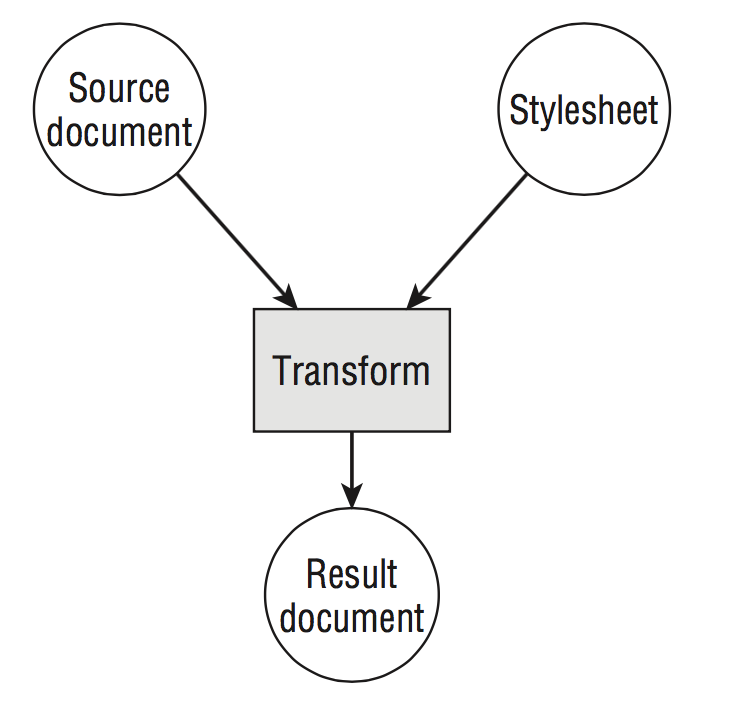
\includegraphics[width=.8\textwidth]{imgs/SchemaXSLTprocessing.png}
    \end{center}
    %\textit{In parte già disponibili nei moduli TEI di base}

\end{frame}

\begin{frame}
    \frametitle{Fondamenti Extensible Stylesheet Language}
    \addtocounter{nframe}{1}
    
    %\begin{center}
    %    
\includegraphics[width=.2\textwidth]{../imgs/tei-r.pdf}
    %\end{center}
    %\textit{In parte già disponibili nei moduli TEI di base}

     \begin{block}{XSL Transformations}
    %     \emph{Per la critica testuale indispensabili i moduli}
         \begin{itemize}
            \item XSLT è un vero e proprio linguaggio di programmazione che usa la sintassi XML
            \item Usa namespace differenti per distinguere fra istruzioni proprie (precedute da \textbf{xsl:}) e output
            \item Legge e scrive alberi XML (ma è possibile ottenere come output anche del
            codice HTML o del testo semplice)
            \item Versione attuale: XSLT 3.0 \url{(https://www.w3.org/TR/xslt-30/)}
        \end{itemize}
     \end{block}
    
\end{frame}

\begin{frame}
    \frametitle{Fondamenti Extensible Stylesheet Language}
    \addtocounter{nframe}{1}
    
    %\begin{center}
    %    
\includegraphics[width=.2\textwidth]{../imgs/tei-r.pdf}
    %\end{center}
    %\textit{In parte già disponibili nei moduli TEI di base}

     \begin{block}{XSL Capacità di trasformazione}
    %     \emph{Per la critica testuale indispensabili i moduli}
         \begin{itemize}
            \item generazione di testo costante;
            \item soppressione del contenuto;
            \item spostamento del testo (es.: scambio ordine di nome e cognome);
        \end{itemize}
     \end{block}
    
\end{frame}

\begin{frame}
    \frametitle{Fondamenti Extensible Stylesheet Language}
    \addtocounter{nframe}{1}
    
    %\begin{center}
    %    
\includegraphics[width=.2\textwidth]{../imgs/tei-r.pdf}
    %\end{center}
    %\textit{In parte già disponibili nei moduli TEI di base}

     \begin{block}{XSL Capacità di trasformazione}
    %     \emph{Per la critica testuale indispensabili i moduli}
         \begin{itemize}
            \item duplicazione del testo (ad es.: tabella di contenuti copiando i titoli);
            \item ordinamento dei contenuti (ad es.: termini in ordine alfabetico);
            \item elaborazione di nuove informazioni in base a quelle esistenti (es. statistiche)
        \end{itemize}
     \end{block}
    
\end{frame}

\begin{frame}
    \frametitle{Fondamenti Extensible Stylesheet Language}
    \addtocounter{nframe}{1}
    
    %\begin{center}
    %    
\includegraphics[width=.2\textwidth]{../imgs/tei-r.pdf}
    %\end{center}
    %\textit{In parte già disponibili nei moduli TEI di base}

     \begin{block}{Caratteristiche fondamentali di XSLT}
    %     \emph{Per la critica testuale indispensabili i moduli}
         \begin{itemize}
            \item Basato su regole di trasformazione (\textit{modello pattern-matching})
            \item Le regole sono dichiarative \textit{(specificano che cosa deve essere generato quando si incontra un certo modello nel documento)}
            \item Le regole possono essere disposte in qualsiasi ordine
        \end{itemize}
     \end{block}
    
\end{frame}


\begin{frame}
    \frametitle{Fondamenti Extensible Stylesheet Language}
    \addtocounter{nframe}{1}
    
    %\begin{center}
    %    
\includegraphics[width=.2\textwidth]{../imgs/tei-r.pdf}
    %\end{center}
    %\textit{In parte già disponibili nei moduli TEI di base}

     \begin{block}{Modalità di Trasformazioni XSLT}
    %     \emph{Per la critica testuale indispensabili i moduli}
         \begin{itemize}
            \item \textbf{Lato server}, utilizzando script Java, ASP, PHP ecc. , per produrre "al volo" pagine HTML sulla base di documenti XML (es. Cocoon);
            \item \textbf{Lato client}, sui Browser che supportano questa tecnologia;
            \item tramite un programma separato (come ad esempio Oxygen), che permette di applicare uno o più scenari di trasformazione.
        \end{itemize}
     \end{block}
    
\end{frame}

\begin{frame}
    \frametitle{Fondamenti Extensible Stylesheet Language}
    \addtocounter{nframe}{1}
    
    %\begin{center}
    %    
\includegraphics[width=.2\textwidth]{../imgs/tei-r.pdf}
    %\end{center}
    %\textit{In parte già disponibili nei moduli TEI di base}

     \begin{block}{Componenti di Base di un foglio XSLT}
    %     \emph{Per la critica testuale indispensabili i moduli}
         \begin{itemize}
            \item Intestazione XML
            \item Elemento radice \textit{stylesheet} e namespace
            \item Eventuali istruzioni di elaborazione
            \item Serie di template rules
        \end{itemize}
     \end{block}
    
\end{frame}

\begin{frame}
    \frametitle{Fondamenti Extensible Stylesheet Language}
    \addtocounter{nframe}{1}
    
    %\begin{center}
    %    
\includegraphics[width=.2\textwidth]{../imgs/tei-r.pdf}
    %\end{center}
    %\textit{In parte già disponibili nei moduli TEI di base}

     \begin{block}{Intestazione XML}
        \texttt{<?xml version="1.0" encoding="UTF-8" ?>}
     \end{block}

     \begin{block}{Elemento radice}
        \texttt{<xsl:stylesheet version='2.0'}
            \\\texttt{  xmlns:xsl='http://www.w3.org/1999/XSL/Transform'>}
     \end{block}
    
\end{frame}

\begin{frame}
    \frametitle{Fondamenti Extensible Stylesheet Language}
    \addtocounter{nframe}{1}
    
    %\begin{center}
    %    
\includegraphics[width=.2\textwidth]{../imgs/tei-r.pdf}
    %\end{center}
    %\textit{In parte già disponibili nei moduli TEI di base}

     \begin{block}{Eventuali istruzioni di elaborazione}
        \texttt{<xsl:output method="xml" version="1.0" indent="yes"/>}
     \end{block}

     \begin{block}{Serie di template rules}
        \texttt{<xsl:template match="/" > ...</xsl:template>} 
        \\\texttt{<xsl:template match="title" > ... </xsl:template>}
     \end{block}
    
\end{frame}

\begin{frame}
    \frametitle{Fondamenti Extensible Stylesheet Language}
    \addtocounter{nframe}{1}
    
    \begin{center}
        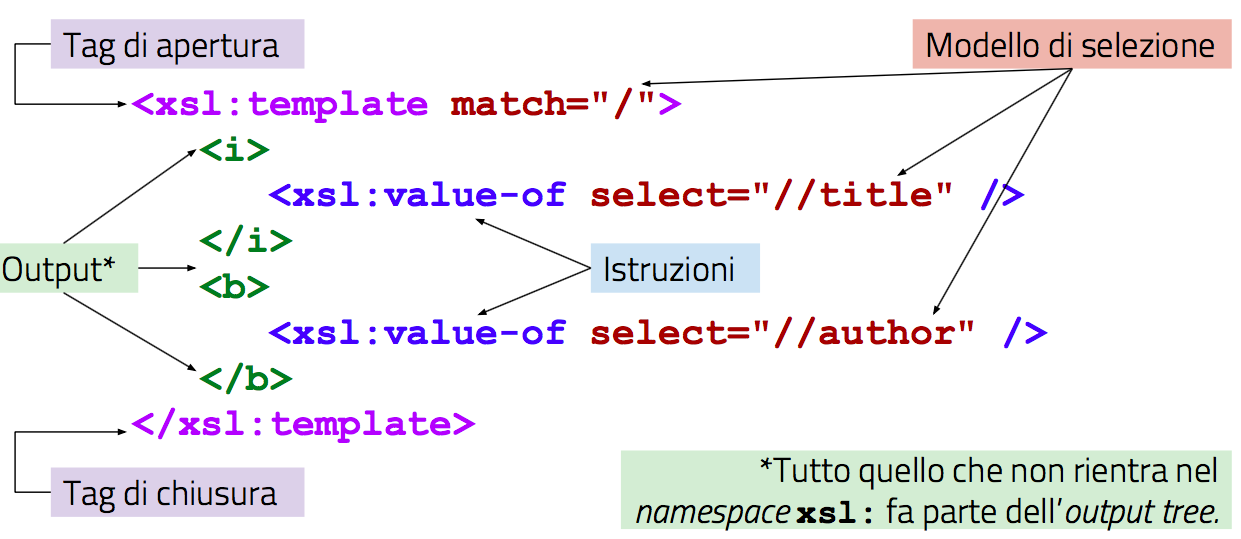
\includegraphics[width=.9\textwidth]{imgs/template-modello.png}
    \end{center}
    %\textit{In parte già disponibili nei moduli TEI di base}

\end{frame}

\begin{frame}
    \frametitle{Fondamenti Extensible Stylesheet Language}
    \addtocounter{nframe}{1}
    
    %\begin{center}
    %    
\includegraphics[width=.2\textwidth]{../imgs/tei-r.pdf}
    %\end{center}
    %\textit{In parte già disponibili nei moduli TEI di base}

     \begin{block}{Come vengono applicate le regole XSLT}
        \emph{Il processore XSLT}
         \begin{itemize}
            \item Legge il documento XML in input e crea l’albero corrispondente
            \item Inizia a percorrere l’albero leggendo i singoli nodi
            \item Confronta ogni nodo con le regole presenti nel foglio di stile
            \item Produce l’output secondo le istruzioni della regola
            \item Restituisce un albero di output
        \end{itemize}
     \end{block}
    
\end{frame}

\begin{frame}
    \frametitle{Fondamenti Extensible Stylesheet Language}
    \addtocounter{nframe}{1}
    
    \begin{center}
        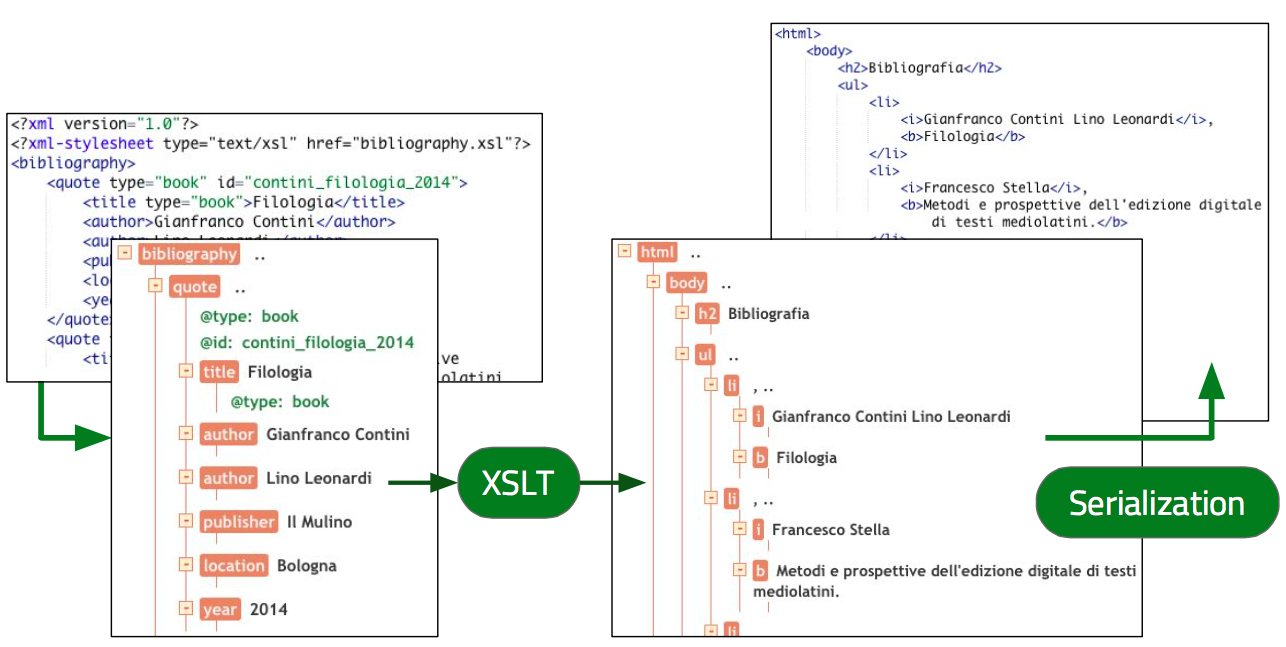
\includegraphics[width=.95\textwidth]{imgs/Processo-xslt.png}
    \end{center}
    %\textit{In parte già disponibili nei moduli TEI di base}

\end{frame}


\begin{frame}
    \frametitle{Fondamenti Extensible Stylesheet Language}
    \addtocounter{nframe}{1}
    
    %\begin{center}
    %    
\includegraphics[width=.2\textwidth]{../imgs/tei-r.pdf}
    %\end{center}
    %\textit{In parte già disponibili nei moduli TEI di base}

     \begin{block}{Esempio di trasformazione}
         Nella sotto-cartella xsl della cartella src leggere il file d'esercizio e individuare le varie componenti.
     \end{block}
    
\end{frame}

\begin{frame}
    \frametitle{Fondamenti Extensible Stylesheet Language}
    \addtocounter{nframe}{1}
    
    %\begin{center}
    %    
\includegraphics[width=.2\textwidth]{../imgs/tei-r.pdf}
    %\end{center}
    %\textit{In parte già disponibili nei moduli TEI di base}

     \begin{block}{Tipi di nodo nell'albero XML}
         \begin{itemize}
            \item \textbf{Radice} del Documento
            \item \textbf{Elementi} con contentuto del sotto albero
            \item \textbf{Attributi}
            \item \textbf{Testo} compresi gli spazi vuoti
            \item \textbf{Commenti} (contenuto tra \texttt{<!-- -->})
            \item \textbf{Namespace} con riferimenti e URI
            \item \textbf{Istruzioni di elaborazione} (contenuto tra \texttt{<? ?>})
        \end{itemize}
     \end{block}
    
\end{frame}

\begin{frame}
    \frametitle{Fondamenti Extensible Stylesheet Language}
    \addtocounter{nframe}{1}
    
    %\begin{center}
    %    
\includegraphics[width=.2\textwidth]{../imgs/tei-r.pdf}
    %\end{center}
    %\textit{In parte già disponibili nei moduli TEI di base}

     \begin{block}{Tipi di nodo nell'albero XML}
         \begin{itemize}
            \item Il \textbf{documento} stesso costituisce la radice (\textit{l'elemento radice XML non è la radice dell'albero di rappresentazione!})
            \item L'intero albero è suddivisibile in sotto-alberi
            \item I nodi più importanti sono gli elementi e i loro attributi
            \item Le entità vengono "tradotte" nel testo loro assegnato al momento
            della dichiarazione
            \item Lo spazio "vuoto" può essere considerato o no
        \end{itemize}
     \end{block}
    
\end{frame}

\begin{frame}
    \frametitle{Fondamenti Extensible Stylesheet Language}
    \addtocounter{nframe}{1}
    
    \begin{center}
        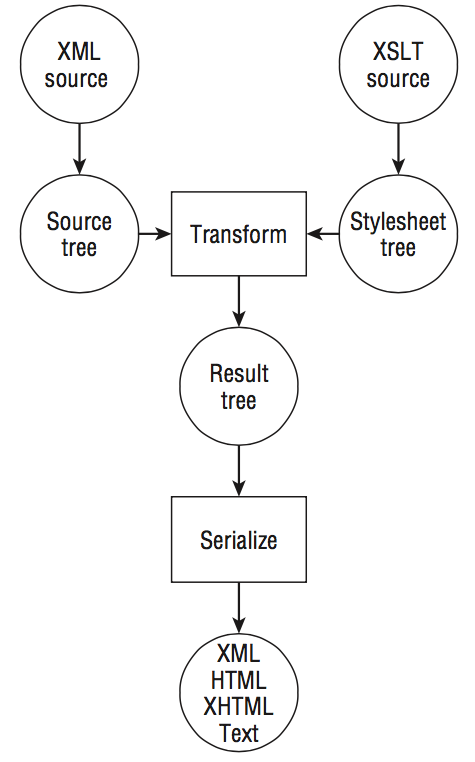
\includegraphics[width=.60\textwidth]{imgs/Schema-trasformazione.png}
    \end{center}
    %\textit{In parte già disponibili nei moduli TEI di base}

\end{frame}

